%%% Important. To have correct table numberings
\renewcommand{\thetable}{\thesection\alph{table}}

\chapter{Excellence}
\label{cha:excellence}

More than a decade after Amazon introduced public cloud services, common sense
is that the public cloud is economical for the consumer, while in reality the
public cloud is economical for the provider.  From the provider perspective the
public cloud is a framework for virtually unlimited and virtually free cloud
resources.

The real revolution that Amazon introduced in 2006 was offering public cloud
services \textbf{to offload the costs of their internal IT}. Amazon was looking
for a solution to a complicated problem: how to meet the widely varying load
requirements of Amazon's virtual store and reduce operational costs at the same
time. Amazon's virtual store peak capacity is hard to predict, and purchasing
servers and data center gear for peak load would be inefficient most of the
time. Offering public cloud services allowed Amazon to have resources for peak
load demands of their virtual store, and to hire out idle resources reducing
operational costs.

If you you can save by consuming cloud services, imagine the possibilities of
\textbf{offloading the costs of your cloud}.  \textit{iWe} offers modular cloud
services that uses Amazon's cost offloading strategy with the convenience and
flexibility of the public cloud, plus the performance, control, and privacy of
internal IT. Our customers get the best of public clouds, the best of internal
IT, and unprecedented economy. We estimate savings for an SME of a factor of 5
compared to public cloud, and of a factor of 15 compared to traditional internal
IT.

\section{Concept}
\label{sec:concept}

\begin{figure}
    \centering
    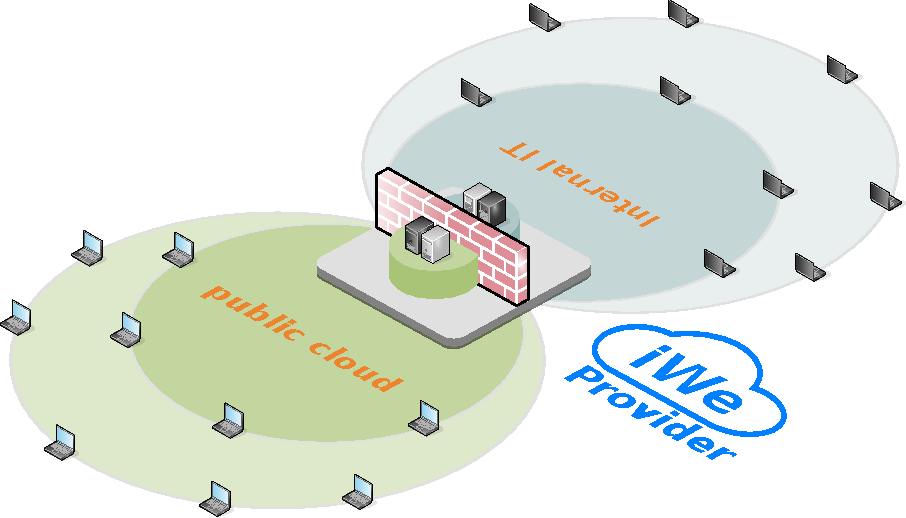
\includegraphics[width=0.7\textwidth]{images/iwe-providers-consumers-with-template2.pdf}
    \caption{SME \textit{iWe Provider}}
    \label{fig:the-clalld-pvt-pub}
\end{figure}

While Internet is becoming essential in virtually all areas of human activities,
cloud computing is pushing Internet away from servers we used to own and
control. One negative result of migrating to the cloud is Internet
centralization, with a few very powerful companies privately owning major shares
of the hardware, software and networks that runs the Internet and stores
\textbf{our} data. With the unbalance between massive providers and
comparatively small consumers, we subject ourselves to services that are
essential to our personal and professional activities, but that may lack
transparency, privacy, control, performance, and a fair price.

We are creating a better cloud, but instead of joining the race for Internet
ownership, instead of building our own massive data centers, we are reverting
the Internet centralization trend by empowering companies (and later will also
empower individuals) from cloud consumers to cloud providers. Our focus on
empowering our community comes from our open source attitude. We are an open
source company, and we are pushing open source ideas to new levels, which is
allowing us to create the first cloud computing sharing economy.

\textit{iWe} will pioneer the sharing economy for cloud computing in a
similar fashion to what Uber does with transport, and to what Airbnb does with
housing. We will start offering public cloud services that are provided by our
community of \textit{iWe Providers} who are the equivalent of Uber drivers,
and Airbnb hosts.

We welcome \textit{iWe Providers} to join us purely for profit, but we expect
to maximize our impact with a different user profile. We expect SMEs to use our
services to get cloud computing resources for their own use, but in better terms
with a transparent service that guarantees technological independence, privacy,
control, performance, and excellent savings. We are confident in our popularity
among SMEs because we offer levels of IT efficiency, convenience, privacy,
and performance that were not previously available to them. We expect SMEs to
use our services to be more competitive, by reducing IT costs, and by getting
more connected computing resources.

As an example, we will describe an SME that joins our community of
\textit{iWe Providers} to get cost-efficient cloud resources for their own
use. This SME has modest needs: 128 GB of RAM, 1000 GB of storage with N+1
redundancy. We opted to demonstrate such as small configuration as we consider
it to be a challenging scenario for efficiency, while common for SMEs
world-wide. Our proposed architecture for this SME is shown on Figure
\ref{fig:the-clalld-pvt-pub} with four physical servers, in two redundancy
pairs, each pair targeting a different audience. The servers run our software
stack which allows us to assume the maintenance responsibility of the entire
environment.

Maintaining the servers of our \textit{iWe Providers} result in a major
advantage: the skills \textit{iWe Providers} need to manage and maintain
their IT lie on the realm of the \textbf{power user} and not the seasoned IT
administrator. As we will show on Table \ref{table:clouds-comparison} of Section
\ref{sec:expected-impact} not requiring systems engineers to maintain the
environment can reduce IT costs.  \textit{iWe} also takes full responsibility
over the public cloud services that we offer but that are provided by our
community of \textit{iWe Providers}. \textit{iWe Providers} don't need to
interact with and worry about consumers for their surplus of server capacity,
and public cloud consumers get a consistent consumer experience from
\textit{iWe}.

Figure \ref{fig:the-clalld-pvt-pub} shows the smallest possible configuration
for an efficient Internal IT capable of high availability, and cost offloading.
The servers on the Internal IT circle are used exclusively by the SME
\textit{iWe Provider} for applications and data that are sensitive in term of
privacy or performance. The other two servers on the public cloud circle provide
the means for offloading costs of the \textit{iWe Provider}. Cost offloading
works in two ways: capacity of these servers is sold as public cloud services on
the \textit{iWe} marketplace and the income is transferred to the SME
\textit{iWe Provider}, and the SME \textit{iWe Provider} can also consume
public cloud resources avoiding additional expenses.

Another characteristic of our service is that we do not charge money from the
\textit{iWe Providers}. Not charging money for our Internal IT service is
core to \textit{iWe} business model, but it doesn't make it a free service.
Instead of charging fees, we exchange our Internal IT service for a share of the
connected computing resources we maintain. This strategy keep the operational
costs low for the \textit{iWe Providers} and give us a building block for our
public cloud services. We sell public cloud services for a profit on our
marketplace closing the loop with income for us.

Our paid public cloud services will start offering regular IaaS with storage,
virtual machines and containers, but with two major advantages: we will offer
extended control over geographical location of resources, allowing deployment in
cities and neighborhoods (instead of continents and countries of current
providers), and the cost structure of \textit{iWe} is efficient. Our business
model allows us to have a massive distributed public cloud without expenses we
would have with traditional data centers. We offload to \textit{iWe
Providers} costs with servers, data center gear, and utility bills, making our
cost structure very efficient.

\section{Positioning of the project}
\label{sec:positioning}

\begin{figure}
\centering
\begin{subfigure}{.5\textwidth}
  \centering
  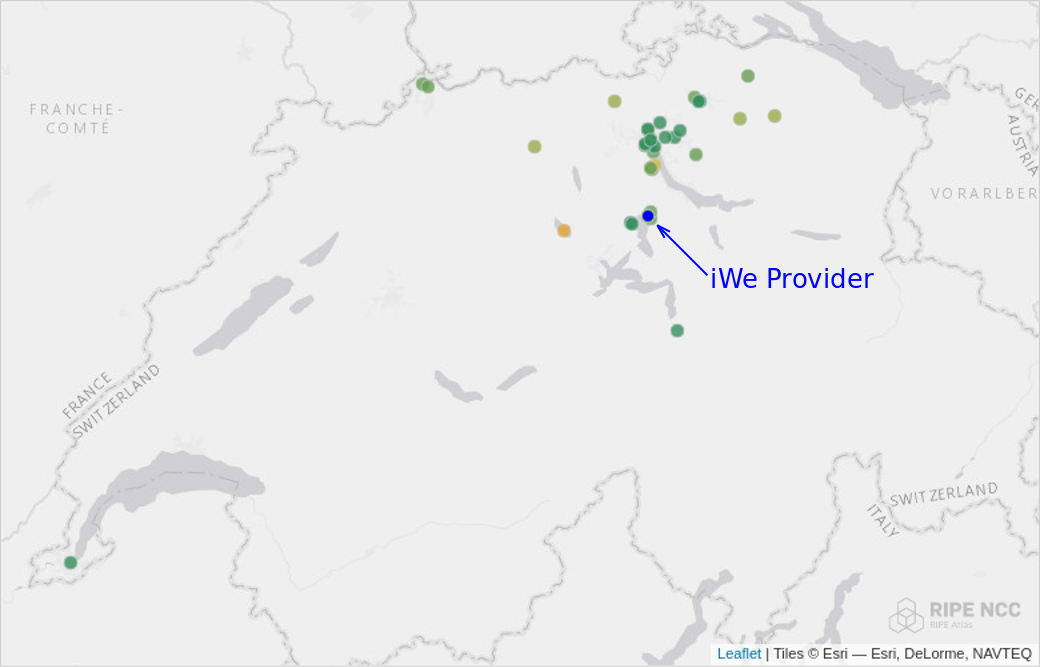
\includegraphics[width=0.98\textwidth]{images/atlas-map.png}
  \vspace{-0.05in}
  \caption{Where are we pinging from}
  \vspace{0.1in}
  \label{fig:sub1}
\end{subfigure}%
\begin{subfigure}{.5\textwidth}
  \centering
  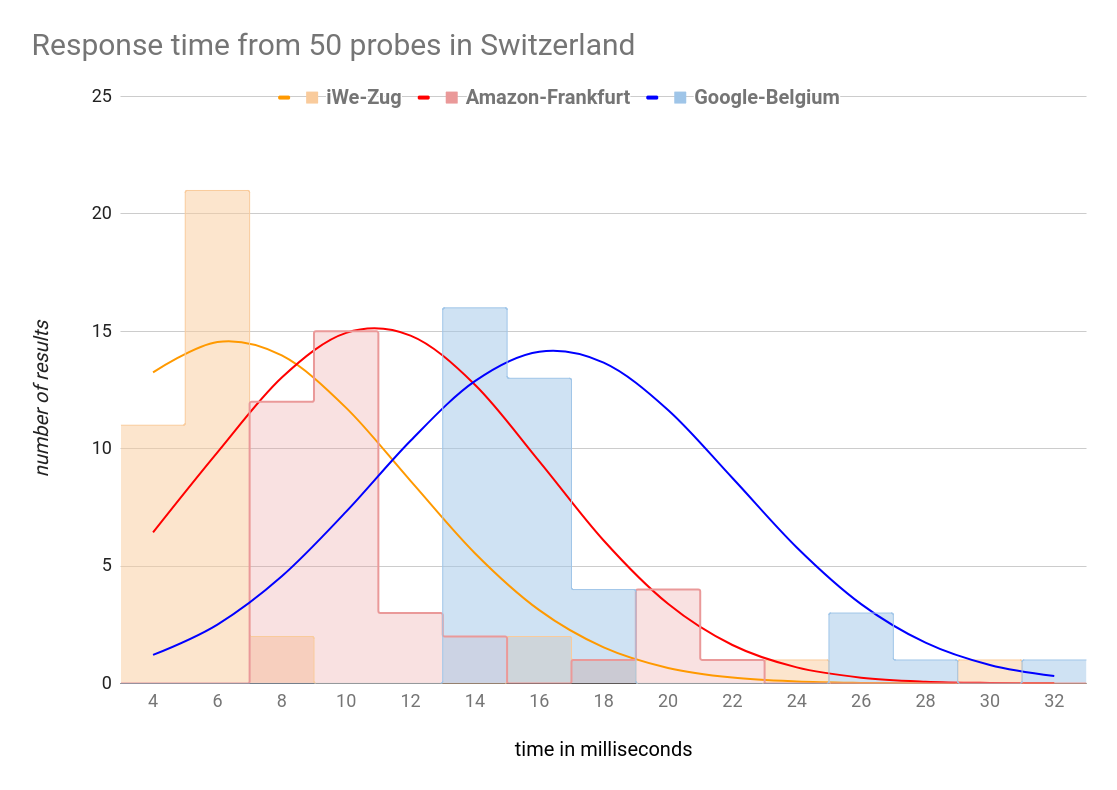
\includegraphics[width=0.96\textwidth]{images/response-time-50.png}
  \vspace{-0.05in}
  \caption{Ping normal distribution and histogram}
  \vspace{0.1in}
  \label{fig:sub2}
\end{subfigure}
  \caption{Details about our latency test}
  \label{latency}
\end{figure}

\begin{table}
    \centering
    \begin{tabular}{r l l l}
                                    & Amazon EC2     & Google Compute & iWe \\
        \hline
        Instance type               &  t2.large & n1-standard-2 & - \\
        \hline

        vCPUs                       &  2 & 2 & 2 \\
        \hline

        Memory                      & 8GB & 7.5GB & 7.5GB \\
        \hline

        Disk                        & 80GiB & 80GB &  80GiB \\
        \hline

        Disk Type                   & GP2 & SSD persistent & SSD persistent \\
        \hline

        Zone                        & eu-central-1b & europe-west1-c & zug-1 \\
        \hline

        Location                    & Frankfurt & Belgium & Zug \\
        \hline

        Monthly cost                & \$ 107.95 & \$ 41.55 & TBD \\
        \hline
    \end{tabular}
    \caption{Specification of the instances}
    \label{table:instances}
\end{table}

We compared the performance of instances running in a very small iWe
provider to instances from Amazon and Google. Table \ref{table:instances} shows
the configuration of each instance, and cost forecast from Amazon and Google.

For Google and Amazon we selected the zones with the lowest latency and higher
bandwidth to our test site in Zug. We used the Network speed test from
CloudHarmony\footnote{https://cloudharmony.com/speedtest-for-aws,
https://cloudharmony.com/speedtest-for-google} to find the zones with better
network performance. All the instances run the same software stack, from the
kernel to the benchmark tools.

We were pinging the instances from 50 different locations in Switzerland as
shown by Figure \ref{latency}(a). Figure \ref{latency}(b) shows the distribution
of results with 82\% of response times for iWe provider in Zug being under 6 ms.
We are using probes from the Ripe Atlas
project\footnote{https://atlas.ripe.net/api/v2/measurements/groups/9229432/} for
our latency test. Figure \ref{graphs}(c) shows the geometric mean of response
times from the probes we are using.

Section \ref{cha:appendix} contains detailed benchmark results for CPU, memory
and IO.

We now plan to extend this benchmark to 10 different locations in Zug,
Switzerland covering different use cases. However full commercialization of
\textit{iWe} will require creation and polishing of web interfaces, server
images, and back end infrastructure.

\section{Ambition}
\label{sec:ambition}

% Explain the novelty of your innovation business project. What do you envisage
% as key market application of the innovation project result?

Section \ref{sec:concept} covered high level overview of the novelty of our
innovation project, key market applications, and the envisaged solution. This
section will describe our potential, and why it is worth to develop and invest
in \textit{iWe}. We will describe opportunities with IoT, the strategy for
our market places, how we plan to gain global traction with local Internet
providers, describe our target relationship with Telecommunication
Companies(Telecoms), and describe our future expansion with home users.

\textbf{IoT} - Peter Levine from Andreessen Horowitz mentioned in a recent
podcast \cite{the-end}: \textit{Cloud computing has pushed computation away from
our own private servers resulting in performance issues related to high latency
between the client and the cloud server. As IoT proliferates, the current model
of cloud computing will become too slow. A small difference in the time it takes
to get a response from the cloud server could be the difference between life and
death in automation for cars and drones.  Computation will move to the edge. In
such an edge computing model, there will be trade of computational resources
without any request to a centralized cloud server.} In the \textit{iWe}
context this excerpt describes how our decentralized architecture will meet IoT
requirements gracefully, as we offer connected computing resources on the edges
of the network, and as we offer a framework for using connected computing
resources as a currency for trade.

\textbf{Marketplaces} - We will have two interconnected marketplaces. The
consumer marketplace is a traditional e-commerce platform that will generate
most of our income by offering services and goods provided by \textit{iWe}
and partners. The services and goods that the consumer marketplace will offer
are defined by our second marketplace, the trusted partner marketplace. We will
offer \textit{iWe} infrastructure and community resources as building blocks
for our partners to create new services, but we will also allow our partners to
create their own customized building blocks. We expect this flexibility to
attract partners that can take advantage of the extended control that
\textit{iWe} offers over the lower software layers of their cloud solution
stack.  As examples, we expect companies such as VMWare, Citrix, SAP, Oracle,
Microsoft, Suse, and Red Hat to offer various services through our trusted
partner marketplace.

\textbf{Global traction} - We offer great cloud solutions to SMEs of all kinds,
but we will start by targeting a specific market niche: Local Internet Service
Providers (LISP). Local means that their service offer is limited to a
geographical area, which is common to providers of Internet access, and of data
center services, such as hosting and co-location. LISPs were popular before cloud
computing, but they are having a hard time competing with giants such as Amazon
and Google. We can help them to regain competitiveness, and to increase revenue
with little effort.  LISP already have the physical infrastructure, including
servers and Internet connection, which will make their gradual transition to
\textit{iWe Providers} easy and cheap. We see LISPs as key partners worldwide
during our first steps on the market.  We will focus on making them an important
share of our early adopters.

\textbf{Telecoms} - With the Internet moving to a few massive data centers, the
role of Telecommunication Companies is rapidly changing from Internet providers
to Internet consumers. One important factor is the loss of corporate customers
to the cloud, which represents services migrating from the Telecom network to
the cloud. One may argue that cloud computing can bring new customers to
Telecoms, however the cloud only brings consumers of the same massive data
centers that were already forcing Telecoms into Internet consumers, speeding up
the transition.  \textit{iWe} offers a shift to the trend of relevance loss,
giving even SMEs the power to host their own services, avoiding moving them to
the cloud or moving them back to the network of their (or our) favorite Telecom.
We also believe we can help Telecoms to sell more connectivity services, and we
expect to develop good partnership with Telecoms worldwide by offering them
highlighted visibility on our marketplaces.

\textbf{The future at home} - We know that enabling individuals to do business
is a powerful strategy that giants such as Uber and Airbnb implement very well.
We want to offer home users a simple way to add resources to the Public
\textit{iWe} for a profit, and expect them to considerably increase our
granularity to support our offer of cloud resources in neighborhoods around the
globe.  We also want to extend the idea of using connected computing resources
as currency for online services, offering \textit{Home iWe Providers}
attractive services to spend their connected resources, instead of simply
trading it all for cash. An example would be to get a premium subscription from
Netflix in exchange for cloud services.
